\documentclass[12pt]{article}
\usepackage{amsmath,amsthm,amssymb}
\usepackage{bm}
\usepackage{hyperref}
\usepackage{color}
\definecolor{darkblue}{rgb}{0,0,0.8}
\hypersetup{
    colorlinks=true,
    linkcolor=darkblue,
    citecolor=darkblue,
    urlcolor=darkblue
}
\usepackage{graphicx}
\usepackage{listings}             % Include the listings-package
\usepackage{tabularx}
\usepackage{longtable}
\usepackage{enumitem}
\usepackage[normalem]{ulem}
\usepackage{pdflscape}
\usepackage{calc}
\usepackage{subfigure}

\definecolor{epcol}{rgb}{0,0, 0.7}
\definecolor{ascol}{rgb}{0 ,0.4, 0}
\definecolor{alertcol}{rgb}{0.7,0, 0}
%\newcommand{\commentas}[1]{{\color{ascol} \footnotesize \it [\marginpar{\bfseries !}AS: #1]}}
%\newcommand{\commentep}[1]{{\color{epcol} \footnotesize \it [\marginpar{\bfseries !}EP: #1]}}
\newcommand{\ascomment}[1]{{\color{ascol} \footnotesize \it [AS: #1]}}
\newcommand{\epcomment}[1]{{\color{epcol} \footnotesize \it [EP: #1]}}
\newcommand{\alert}[1]{{\color{alertcol} #1}}
\newcommand{\as}[1]{\marginpar{\bfseries !}{\color{ascol} #1}}
\newcommand{\ep}[1]{\marginpar{\bfseries !}{\color{epcol} #1}}
\newcommand{\epdel}[1]{{\color{epcol} \sout{#1}}}
\newcommand{\asdel}[1]{{\color{ascol} \sout{#1}}}

\usepackage[paperwidth=187.5mm, paperheight=265.179mm, left=0.5in, top=0.75in, right=0.5in, bottom=0.5in, includefoot]{geometry}
 % this is for the convenience of A.S. 

% Standard commands

\newcommand{\ai}{{\rm ai}}
\renewcommand{\_}{\char`_}
\newcommand{\eps}{{\epsilon}}

\bibliographystyle{abbrv}

\author{Alexander V. Shapeev (e-mail: \texttt{a.shapeev@skoltech.ru})
\\
Evgeny V. Podryabinkin (e-mail: \texttt{e.podryabinkin@skoltech.ru})
\\
Ivan S. Novikov (e-mail: \texttt{i.novikov@skoltech.ru})
}

\title{MLIP: a user %and developer 
manual}
\begin{document}\sloppy

\lstset{language=C++, basicstyle={\small\ttfamily}}  
\maketitle

\begin{abstract}
	MLIP is a software package implementing several machine learning interatomic potentials (aka force fields) for calculating the energy, forces and stresses of atomic configurations.
	Such potentials seek to combine the accuracy of quantum mechanics with the computational efficiency of the empirical potentials.
	%The structure and algorithm of the MLIP are described in \cite{Shapeev2016-MTP}
\end{abstract}


\tableofcontents

%\pagebreak

\section{Some important info}
\subsection{Status of this document}	
This manual was written for the first (one-component) version of this software and has not been updated much.
If something written here does not work then please refer to \texttt{test/examples/} to see how things should work.

\subsection{Licensing and distribution}	
This package is developed by the group of Alexander Shapeev (\texttt{a.shapeev@skoltech.ru}) at Skoltech (Skolkovo Institute of Science and Technology), Moscow, Russia.
To use this software you are obliged, in short, not to distribute it, to use it only for noncommercial research and to acknowledge its use by properly citing the work.
See the \texttt{LICENSE} file for the details.

\subsection{A Quickstart guide (aka TL;DR)}

You like pushing buttons but not reading long texts?
Try:
\begin{itemize}
\item Download the source through git by executing
\\[0.5em]
$\mathstrut$~~~~\texttt{git clone \url{http://gitlab.ru/shapeev/mlip-2.git mlip}}
\\[0.5em]
This will create the \texttt{mlip/} folder with the sources.

\item Install: Execute \texttt{make mlp} in the \texttt{make/} folder to build the \texttt{mlp} tool. Run the shell script in \texttt{make/LAMMPS/} to install MLIP with LAMMPS. The \texttt{lmp\_serial} and \texttt{lmp\_mpi} binaries will be created in the \texttt{LAMMPS/src/} folder and copied over to the \texttt{make/} folder.

\item Try out examples, see \texttt{doc/examples/readme.txt}.
\end{itemize}

\section{Theory}\label{sec:theory}

You are advised to read Section \ref{sec:theory:basic}, but you can skip the rest of Section \ref{sec:theory} if you have read \cite{Shapeev2016-MTP,podryabinkin2017-AL,gubaev2018-mtp-multicomponent}.

\subsection{Basic terms and definitions}\label{sec:theory:basic}

\begin{itemize}
	\item In this document, we will refer to this package as \emph{MLIP}, while the machine learning interatomic potentials will be just called ``machine learning potentials'' or just ``potentials''. 
	
	\item The empirical (classical) interatomic potentials, such as Lennard-Jones or EAM, will be specifically referred to as the \emph{empirical potentials}.
	
	\item \emph{Ab initio model} (AIM) means any interatomic interaction model or potential which is considered to reproduce sufficiently accurately the behavior of the real atomic systems. Such models are typically computationally expensive. The main examples are Density Functional Theory (DFT), Orbital-free DFT, Hartree-Fock, etc.
	This package allows for using LAMMPS as an ab initio model.
	
	\item We will call an atomistic \emph{configuration} a system with $N$ atoms described by a collection of their types (presently, MLIP handles configurations with only one type, i.e, single-component configurations), their positions, and the supercell given by three lattice vectors ($L = \big(l_1 \,\, l_2 \,\, l_3\big)\in{\mathbb R}^{3\times 3}$).
	A configuration is typically denoted by $x$.
	The supercell, thus, defines the periodic boundary conditions.
	A very large supercell can be given to simulate non-periodic boundary conditions.
	
	\item The \emph{neighborhood} of atom $i$, $1\leq i\leq m$, is defined as a collection (tuple) of vectors pointing from atom $i$ to all the atoms and their periodic extensions, excluding the atom itself, that are not farther than $R_{\rm cut}$ (inside a cutoff sphere).
	
	\item The ``EFS'' abbreviation will be used for the collection of the energy $E(x)$, forces $(f_i(x))_{1\leq i\leq N}$ acting on atoms, and stresses $\sigma(x)=(\sigma_{ij}(x))_{1\leq i,j\leq 3}$ of the atomic configuration $x$.
	
	\item We will use the term \emph{driver} as the algorithmic component of an atomistic simulation that generates a set (or a sequence) of configurations.
	The examples of drivers are: molecular dynamics (MD), structure relaxation, Monte-Carlo sampling, nudge elastic band, etc.
	Also, reading configurations from database is also considered a driver in MLIP.
\end{itemize}

\subsection{Machine learning potentials}

The main purpose of machine learning potentials is to reproduce the behavior of ab initio models (AIMs) at a tiny fraction of the computational cost.
Machine learning potentials postulate a partitioning of energy into individual contributions of atoms, each contribution depends on the neighborhood of the atom, and assume a flexible functional form for such contributions depending on the positions and types of surrounding atoms within a certain cutoff radius, typically with hundreds or more parameters. These parameters are found by requiring the energy, forces and/or stresses predicted by a potential to be close to those obtained by an AIM on some atomic configurations. These configurations are called the \emph{training set}, and finding the parameters of a potential is known as \emph{training} or \emph{fitting}. One of the important features (requirements) of a potential is its ability to approximate potential energy surfaces with an arbitrary accuracy (at least theoretically) by increasing the number of parameters and the training set. Due to this, one can improve the accuracy of the potential at the cost of reducing its computational efficiency and vice versa.

\subsection{Moment tensor potentials}

Moment Tensor Potentials (MTPs) \cite{Shapeev2016-MTP} are machine learning potentials implemented in the MLIP package. MTPs adopt a linear regression model with polynomial-like functions of atomic coordinates as the basis functions.
Potential energy (contribution) of an atom (site energy) provided by MTP as a function of atomic environment within a cutoff sphere (neighborhood) is invariant with respect to all Euclidian transformations and permutations of the chemically equivalent atoms. It has been proved theoretically and shown computationally that MTP allows for systematically improving the accuracy by increasing the number of basis functions.

MTP has a complex functional form that depends on the number of parameters and the particular basis functions.
Therefore MTPs, as a rule, can not be written in a plain compact form and require a complex algorithms for their efficient evaluation and fitting.
Such algorithms are implemented in MLIP.
The current implementation of MTPs is limited to systems with one atomic type.

\subsection{Fitting}

Mathematically, training (fitting) of a potential is determining its unknown parameters from a (typically, overdetermined) system of linear equations, which expresses that the energy, forces and stresses (EFS in short) predicted by the potential are close to the given (ab initio) ones:
\begin{align*}
E\big(x^{(k)}\big) &= E^\ai\big(x^{(k)}\big)
\\
f_i\big(x^{(k)}\big) &= f_i^\ai\big(x^{(k)}\big), \quad {1\leq i\leq N^{(k)}}
\\
\sigma\big(x^{(k)}\big) &= \sigma^\ai\big(x^{(k)}\big)
\end{align*}
for the configuration $x^{(k)}, {1\leq k \leq K}$ from the training set \cite{Shapeev2016-MTP, ActiveLearning}.

The EFS enter the least squares functional with different coefficients:
\begin{equation}
\label{eq:fit}
\begin{split}
\sum_{k=1}^K\Big[~~~&\frac{C_E}{N^{(k)}} \Big(E\big(x^{(k)}\big)-E^\ai\big(x^{(k)}\big)\Big)^2 ~~+\\
+~~&C_f \sum_i^{N^{(k)}} \Big|f_i\big(x^{(k)}\big)-f_i^\ai\big(x^{(k)}\big)\Big|^2 ~~+ \\
+~~&\frac{C_\sigma}{N^{(k)}} \sum_{i,j=1}^3  \Big(\sigma_{ij}\big(x^{(k)}\big)-\sigma^\ai_{ij}\big(x^{(k)}\big)\Big)^2 ~~ \Big] \longrightarrow \min,\\
\end{split}
\end{equation}
where $N^{(k)}$ is the size of (i.e., the number of atoms in) $x^{(k)}$.
Note that the scaling by $N^{(k)}$ is chosen so that the same configuration with a larger unit cell has the same relative contributions of EFS.
The coefficients $C_E$, $C_f$, $C_\sigma$ are the adjustable parameters of the fitting.
The default values are $C_E = 1$, $C_f = 0.01 {\rm \AA}^2$, $C_\sigma = 0.001$.

\medskip
There is an alternative form of fitting, where the small forces are fitted more accurately than the large 
\begin{equation}
\label{eq:fitrel}
\begin{split}
\sum_{k=1}^K\Big[~~~&\frac{C_E}{N^{(k)}} \Big(E\big(x^{(k)}\big)-E^\ai\big(x^{(k)}\big)\Big)^2 ~~+\\
+~~&C_f \sum_i \frac{\big|f_i\big(x^{(k)}\big)-f_i^\ai\big(x^{(k)}\big)\big|^2}{\big|f_i^\ai\big(x^{(k)}\big)\big|^2+\eps_f^2}~~+ \\
+~~&\frac{C_\sigma}{N^{(k)}} \sum_{i,j=1}^3  \Big(\sigma_{ij}\big(x^{(k)}\big)-\sigma^\ai_{ij}\big(x^{(k)}\big)\Big)^2 ~~ \Big] \longrightarrow \min,\\
\end{split}
\end{equation}
where $\eps_f$ is an additional adjustable parameter.

\subsection{Active learning}

There are two approaches to the fitting of the potentials, known as passive learning and active learning (AL).
In contrast to passive learning in which a potential learns every configuration in the training set, the concept of active learning assumes some algorithm analyzing and selecting an optimal (D-optimal) training subset \cite{ActiveLearning}. The key component of any AL method is, thus, its \emph{query strategy}---an algorithmic criterion for deciding whether a given configuration should be added in the training subset. 
The query strategy does not use ab initio EFS (otherwise the whole purpose of AL is defeated).

There are three query strategies currently implemented in MLIP based on an estimate of degree of extrapolation when a machine learning potential is used for calculation of (1) configuration energy, (2) site energy of atomic neighborhoods, and (3) forces and stresses.
It has been shown that active learning does not lead to a decrease of approximation accuracy (moreover the maximal errors typically diminish) whereas its transferability (i.e. ability to predict EFS reliably outside the training domain) improves.

\subsection{Learning on the fly}

Active learning is the key component of our version of learning on the fly, where the training set selection, the fitting of the potential, and an atomistic simulation are combined in a single process (learning on the fly is schematically shown in Fig.\ \ref{fig:LOTF}).
%Selection of configurations on the fly and learning on the fly are the features of this package. 

\begin{figure}[htbp]
	\centering
	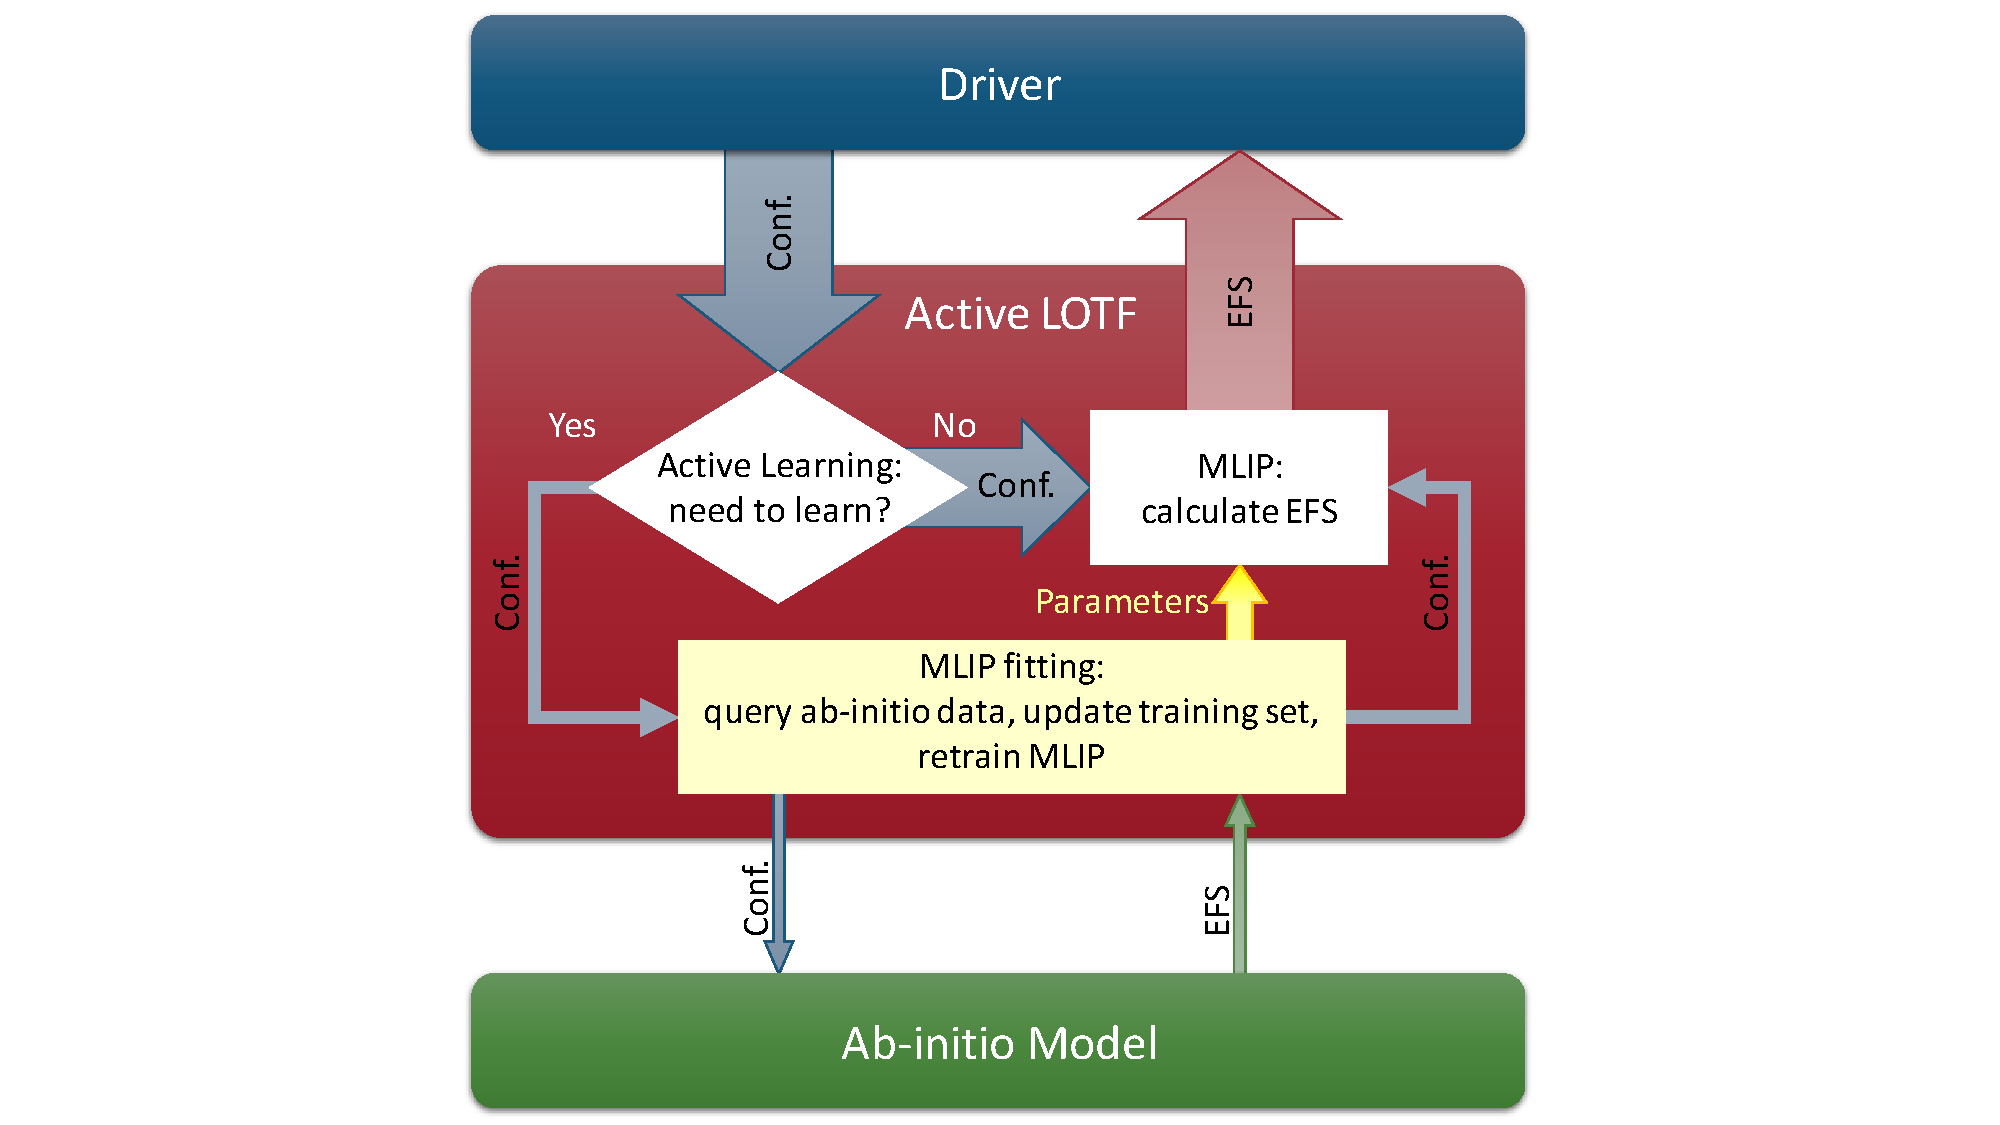
\includegraphics[width=4.0in]{figs/LOTF.pdf}
	\caption{Workflow in actively learning a potential on the fly.
		In the course of iterations an AL potential receives from MD a configuration and estimates the reliability of EFS calculation.
		If it detects sufficient extrapolation when calculating EFS, MLIP queries ab initio EFS, add this configuration to the training set, and retrains the potential.
		Then it calculates the EFS and passes it to the driver.
	}
	\label{fig:LOTF}
\end{figure}

\section{MLIP concept} \label{sec:concept}

MLIP, roughly speaking, provides tools for fitting potentials and using them in atomistic simulations.
MLIP, thus, can be used:
\begin{itemize}
\item
as a stand-alone package \texttt{mlp}, allowing for fitting the potentials and doing some simple atomistic simulations (see Section \ref{sec:install:mlp} for installation), and

\item as a plugin for external molecular modeling codes, like LAMMPS --- refer to the \texttt{INSTALL.md} file.
\end{itemize}

\begin{figure}
\begin{center}
\hfill
\subfigure[fitting on a database\label{fig:diagrams:fit}]{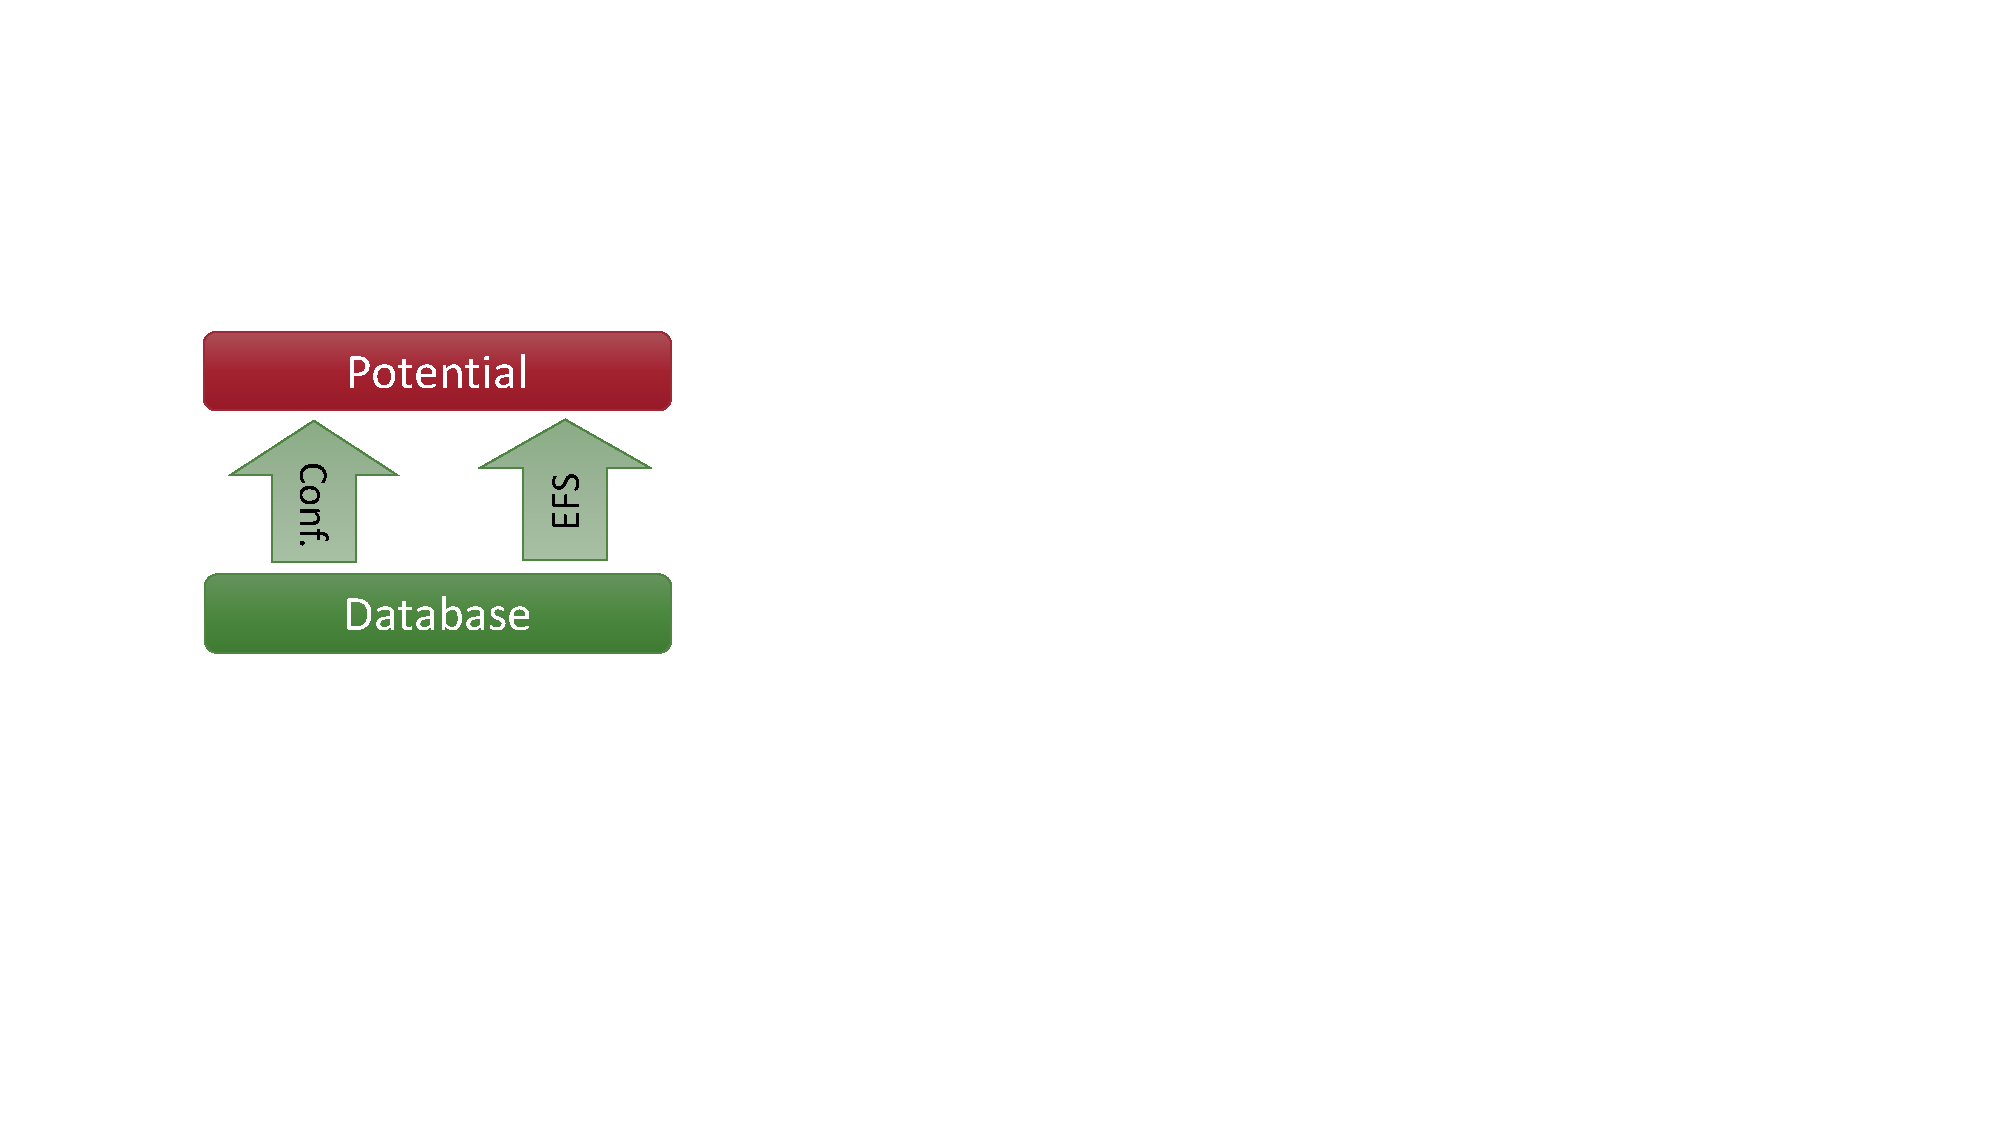
\includegraphics[page=1,scale=.5]{figs/diagrams.pdf}}
\hfill\hfill
\subfigure[simple atomisitic simulation\label{fig:diagrams:simple}]{\includegraphics[page=2,scale=.5]{figs/diagrams.pdf}}
\hfill\hfill
\subfigure[a learning-on-the-fly simulation\label{fig:diagrams:lotf}]{\includegraphics[page=3,scale=.5]{figs/diagrams.pdf}}
\hfill$\mathstrut$
\end{center}
\caption{Diagrams showing different ways of using MLIP: fitting and atomistic simulation.}
\label{fig:diagrams}
\end{figure}

The following is the typical use cases of MLIP:
\begin{itemize}
\item[(a)]
Fitting a potential on a configuration database (see Figure \ref{fig:diagrams:fit}).
This is achieved through \texttt{mlp train}.
The fitting errors (and validation errors) can be computed using \texttt{mlp calc-errors}.

\item[(b)]
A simple atomistic simulation with a trained potential (see Figure \ref{fig:diagrams:simple}).
Typically, this is done through LAMMPS.

\item[(c)]
A learning-on-the-fly type of simulation (see Figure \ref{fig:diagrams:lotf}).
This can be done both, through LAMMPS and \texttt{mlp run}.
\end{itemize}

In fact, the scenario (c) encompasses all the other scenarios (at least in the serial version of MLIP).
For example, (b) corresponds to (c) when Potential decides not to do any ab initio calculations, while (a) corresponds to (c) when Driver=``reading from a database'' and AIM=``preserve EFS as read from the database''.

More details are given in Section \ref{sec:aim}.

\section{Installation} \label{sec:install}

MLIP uses OpenBLAS (\url{http://www.openblas.net}) as a static library and is distributed as a part of this package (namely, OpenBLAS v.0.2.19 in the \texttt{blas/} folder). MLIP's makefile is configured to build and link to it automatically; if you want to link to your version of BLAS (for any reason) you should modify the makefile accordingly. 

MLIP can be build and used (1) as stand-alone package; and (2) as a part of LAMMPS. 


\subsection{Building as a stand-alone package}\label{sec:install:mlp} 

Let \texttt{MLIP/} be a directory with MLIP sources pulled from \url{http://gitlab.skoltech.ru/shapeev/mlip}. 

\begin{enumerate}
	\item Specify your C++ compiler in the makefile:
	
		\subitem In the makefile (located in \texttt{MLIP/make/}) specify the compiler supporting the \texttt{C++11} standard (in a line beginning with ``\texttt{CC =}''). The default is \texttt{g++}.
	
	\item In the directory \texttt{MLIP/make/} build MLIP by executing \texttt{make mlp}.
	The executable \texttt{mlp} should then appear in the same directory.
\end{enumerate}

\subsection{Building on Windows}

Visual Studio projects of MLIP are available in \texttt{MLIP/dev/} folder.


\section{Usage examples} \label{Using}

The examples demonstrate the most frequently used routines. Each example contains a brief description in the \texttt{readme.txt} file, the input files, the settings file \texttt{mlp.ini} and the expected output in the \texttt{sample\_out} folder.
The output (normally) is written to the \texttt{out/} folder.
All examples are available in \texttt{MLIP/doc/examples/}.

\section{MLIP file formats}

\subsection{Internal format of configuration files}\label{cfg-file}

MLIP supports two internal formats for storing configurations in database files, typically having the ``\texttt{.cfg}'' extension: textual and binary.
We recommend using the binary format when the speed of input/output operations is critical.
The textual format, in contrast, is useful when configurations are prepared manually or converted from an unsupported format.

The example of configuration in the textual file format is bellow:

{\small
	\begin{verbatim}
	BEGIN_CFG
	 Size
	     12
	 Supercell
	        5.804540      0.000000      0.000000
	       -0.000052      4.304488      0.000000
	 AtomData: id type  cartes_x  cartes_y  cartes_z        fx        fy        fz
	            1    0  -0.06668   1.48178   2.12328   0.00116   0.00035   0.00023
	            2    1   1.23010   2.65535   1.49390  -0.00259  -0.00072   0.00170
	            3    0  -0.54459   4.36682   3.13176   0.00168   0.00059   0.00035
	            4    0   3.12308   2.65537   1.51976  -0.00075   0.00044  -0.00077
	            5    0   4.41954   1.48201   0.89064   0.00001  -0.00156  -0.00136
	            6    1   3.58878   3.89084   2.64425   0.00008   0.00077  -0.00044
	            7    0   3.44883   4.27728   0.83155   0.00105   0.00136   0.00081
	            8    0   0.46582   2.80689   3.10745  -0.00320  -0.00174  -0.00034
	            9    0   0.76409   3.89093   0.36959  -0.00025  -0.00035  -0.00032
	           10    1   3.30134   2.21479   3.25088   0.00283  -0.00171   0.00059
	           11    0   0.90387   4.27708   2.18219   0.00016   0.00292  -0.00053
	           12    0   2.29143   4.95920   3.27520  -0.00019  -0.00036   0.00006
	 Energy
	        -76.697992341920
	 Stress:  xx          yy          zz          yz          xz          xy
	    -0.00121     0.00075     0.00233     0.00191     0.00246    -0.00156
	 Feature    EFS_by    VASP
	 Feature    from      relaxation_driver
	 Feature    min_dist  1.734226
	 Feature    type_0    B
	 Feature    type_1    Al
	 Feature    comment	  
	 Feature    comment	   ((`'-"""-'`))
	 Feature    comment	    )  -   -  (
	 Feature    comment	   /   o _ o   \
	 Feature    comment	   \   ( 0 )   /
	 Feature    comment	    '-.._^_..-' 
	END_CFG
	\end{verbatim}
}

The description of each configuration in the database starts with \texttt{BEGIN\_CFG} and ends with \texttt{END\_CFG}. No symbols except whitespace (which is space, tab, and the newline characters '\textbackslash n' and '\textbackslash r') are allowed between configurations.
After \texttt{BEGIN\_CFG} several compulsory and optional fields follow. Bellow is the list of recognizable fields. 
\begin{enumerate}
	\item \texttt{Size} (compulsory field) is followed by one integer number, the number of atoms in the configuration.
	\texttt{Size} should appear before ``\texttt{AtomData:}''.
	
	\item \texttt{Supercell} (optional field) is followed by 3, 6, or 9 numbers, the 3 coordinates of the first lattice vector, then (optionally) 3 coordinates of the second lattice vector, and (optionally) 3 coordinates of the third lattice vector. 
	If \texttt{Supercell} is missing then no lattice vectors are given (this is a open-shell molecule).
	
	\item ``\texttt{AtomData:}'' (compulsory field) contains the per-atom data (atomic coordinates, forces, atom types, etc.). 		\texttt{AtomData:} is followed by one or more field names (on the same line):
	\begin{enumerate}
		\item \texttt{id} (optional field) means the ordinal number of atom in the configuration (1, 2, ...). If \texttt{id}'s are given, but are different from 1, 2, 3 in exactly in this order, it is an error.
		\item \texttt{type} (optional field) are the element types (0, 1, \ldots); if they are empty then all atoms are considered as of $0$ type and this is a single-component configuration.
		\item \texttt{cartes\_x}, \texttt{cartes\_y}, \texttt{cartes\_z} (all three are compulsory fields) means the Cartesian coordinates (measured in \AA).
		There is an alternative option to provide the configuration with direct (fractional) coordinates. In this case \texttt{direct\_...} caption should be specified instead of \texttt{cartes\_...}.
		\item \texttt{fx}, \texttt{fy}, \texttt{fz} (optional fields, but all three are required if present), are the force components in Cartesian coordinates (measured in eV/\AA).
		\item \texttt{site\_en} (optional field) is the site energy (in a rare occasion it is defined). 
		\item \texttt{charge} (optional field) may be used for storing of atomic partial charges.
	\end{enumerate}

	\item \texttt{Energy} (optional field) is followed by one number (measured in eV). 
	
	\item ``\texttt{Stress:}'' (optional field) must be immediately (on the same line) followed by the following 6 (not more and not less) field names (in any order), \texttt{xx}, \texttt{yy}, \texttt{zz}, \texttt{yz}, \texttt{xz}, and \texttt{xy}.
	On the next line are the 6 numbers, corresponding to those stresses.
	These are virial stresses multiplied by the cell volume (measured in eV).
	Positive stresses correspond to over-stretched configurations (in other words, ``stress = $-$force on the supercell'')
	
	\item ``\texttt{Feature}'' (optional fields, multiple entries are allowed) is/are additional (textual) attributes of a configuration (such as what chemical elements corresponds to the atom indexes, what generated it, what computed its energy, whether it is an ideal crystal or has a defect, etc.). Each ``Feature'' has a name (one word without whitespace) and value (a string separated from the name by a space or a tab character). A configuration may contain several features. 
	If two lines with the same name appear, the newline (`\texttt{\textbackslash n}') character and the second line are appended to the first line; similarly for the third line, etc.
	The features do not have universal meanings, they are used by different tools.
\end{enumerate}


\subsection{MTP file}\label{MTPfile}

The functional form of MTP and, optionally, the parameters are encoded in the \texttt{.mtp} files.
% MLIP is able to handle files of this type constructing machine representation of the MTP. Using machine learning potentials is possible after loading from the appropriate file (it also possible to save the potential after fitting).
MTPs may differ by:
\begin{itemize}
	\item particular basis functions of the atomic environment;
	\item the number of basis functions;
	\item the minimal allowed interatomic distance;
	\item the cut-off radius;
	\item values of the parameters.
\end{itemize}
Some of these properties can be seen directly in an \texttt{.mtp} file, and the minimal and cutoff distances can be edited directly (if you do it you have to re-train the potential).
Fitted MTPs can be distinguished from the non-fitted ones by the presence of the ``\texttt{moment\_coeffs}'' string followed by the list of parameters in the \texttt{.mtp} file.

\subsection{Settings file}
MLIP can be configured to work with external codes, learn on the fly, etc.
These settings are the given in the settings file (typically \texttt{mlip.ini}) and are described in Section \ref{Settings}.


\section{A driver-potential-AIM framework}\label{sec:aim}

Many use cases fall into the driver-potential-ab initio model framework as described below.
The interaction between an atomistic simulation (driver) and MLIP can be viewed as the following data exchange (according to the scheme shown in Fig.~\ref{fig:diagrams:lotf}): 
\begin{enumerate}
	\item the driver generates a configuration and passes it to the model;
	\item the model optionally queries EFS for this configuration from the ab initio model;
	\item the model calculates EFS for this configuration and passes it to the driver;
	\item the driver processes EFS data from the model and generates new (or modify in some way) the configuration and repeats the first step.
\end{enumerate}

This scheme obviously describes the plain atomistic simulation scenario (with no communication between MLIP and ab initio model) and the learning-on-the-fly scenario.
Fitting and active learning from the database are also described by this scheme when the driver simply reads configurations from a database while the ab initio model simply returns the EFS data that are read from the database.
This point of view unifies many typical operations with configurations and machine learning potentials into the general scheme shown in Figure \ref{fig:diagrams:lotf}. 

The particular operational mode of MLIP is determined from the input settings file. The scope of the main operations with configurations and machine learning potentials determining the mode are listed in Section~\ref{Capabilities}, the structure of the settings file is described in Section~\ref{Settings}. 

%\begin{figure}[htbp]
%	\centering
%	\includegraphics[width=2in]{figs/Diagram.pdf}
%	\caption{ General scheme of MLIP functioning: MLIP receives configuration from the driver, process it according with the set operating mode, optionally query EFS data for this configuration from the ab initio model (it can be needed, for example, for training the potential or calculation of approximation errors) and returns the EFS to the driver. 
%	Driver considers MLIP as the interatomic interaction model (treated as a blackbox) for EFS calculation. }
%	\label{fig:Diagram}
%\end{figure}

Generally the driver is some external package which uses MLIP as interatomic interaction model, however MLIP has two embedded drivers: (1) reading configurations from a database file and (2) relaxation (Section~\ref{internal_drivers}). When MLIP is operating under external driver it should be compiled as a part of the package providing that driver. This version of MLIP distributive provides an interface to LAMMPS package (see Section~\ref{sec:install} describing compiling the joint software and Section~\ref{lammps_drivers} describing MLIP usage from LAMMPS). 

MLIP also supports working with a number of internal and external EFS calculators:
\begin{enumerate}
	\item DFT by VASP (external), see Section~\ref{abinitio} for more details;
	\item any empirical potential available in LAMMPS (external) described in the Section~\ref{abinitio};
	\item Lennard-Jones potential, usually used for testing purposes (internal);
	\item internal dummy EFS ``calculator'', keeping the EFS data provided with the configurations in a database file;
	\item another well-trained machine learning potential, which can be used, for example, for the fitting of ``light'' potentials (internal).
\end{enumerate}
Communication between MLIP and external EFS calculators is implemented through the exchange of files. Internal AIMs are set in the settings file (details of configuring are given in Section~\ref{abinitio}).

In addition, MLIP provides a set of tools for self-testing, converting files into the ``.cfg'' format (for more details about the format see Section~\ref{cfg-file}), parallel MTP fitting and parallel error calculation. These tools can be executed from the command line. All tools are described in a detail in Section~\ref{utils}.

\subsection{Capabilities of MLIP}\label{Capabilities}

MLIP is a multifunctional tool communicating with a driver and an AIM as shown in Fig.\ \ref{fig:diagrams}.
A particular operational mode is fully determined by the combination of the following options (each can be enabled or disabled independently from others).
\begin{itemize}
	\item[O1.] Calculation EFS for the configurations provided by the driver.
	\item[O2.] Learning on the configurations (EFS for these configurations are queried from the ab initio model).
	\item[O3.] Active selection of the configurations provided by driver;
	\item[O4.] Comparison of EFS calculated by the potential and the AIM and accumulation of the average errors of approximation;
	\item[O5.] Writing the processed configurations to a file (together with the EFS that are passed to the driver);
	\item[O6.] Writing the log with the following information: the total number of configurations processed to the moment, the number of ab initio and MTP calculations of EFS.
\end{itemize}
All these options also have their own settings and parameters (that are described in detail in Section~\ref{Settings}).
Table~\ref{tab:regimes} presents the most important scenarios that are defined by the combination of O1, O2 and O3. Options O4, O5, O6 provide the scenarios 1--8 from Table~\ref{tab:regimes} with the additional functionality but do not change the scenarios themselves.

\begin{table}[htbp]	\small
	\centering
	\caption{Description of the main scenarios defined by the combination of O1, O2 and O3 options}
	\medskip
	\label{tab:regimes}
	\begin{tabular}{c|c|c|c|p{.60\textwidth}}
		     & Calc. &       &        &  \\
		Mode & EFS   & Learn & Select &  \\
		     & (O1)  & (O2)  & (O3)   & Scenario description\\
		\hline
		1&no&no&no& EFS is calculated by AIM. No action is performed with MTP.\\[.5em]
		
		2&yes&no&no& Calculation mode. MLIP just calculates EFS by MTP for each configuration provided by the driver.\\[.5em]
		
		3&no&yes&no& Learning mode.
		MLIP fits MTP (according to the fitting settings) on the all the configurations provided by driver.
		The training is done on EFS provided by the AIM.
		The same EFS are returned to the driver.
		\\[.5em]
		
		4&no&no&yes& Selection mode.
		MLIP just selects (according to the selection settings) a D-optimal set of the configurations among all those provided by driver.
		EFS returned to the driver depend on the setting \texttt{mlip:select:efs\_ignored}: if false then the EFS are taken from the AIM, otherwise EFS have unpredictable values (see Section~\ref{Settings} for more details).\\[.5em]
		
		5&yes&yes&no& Learning and calculation mode. The same as 3,
		but the EFS are calculated by MTP and returned to the driver.\\[.5em]
		
		6&yes&no&yes& Selection and calculation mode. The same as 4, but the EFS are calculated by MTP and returned to the driver.\\[.5em]
		
		7&no&yes&yes& Active learning mode.
		MTP is fitted on a D-optimal training set (according to the selection and fitting settings).
		EFS returned to the driver depend on the setting \texttt{mlip:select:efs\_ignored}: if false then the EFS are taken from the AIM, otherwise EFS have unpredictable values (see Section~\ref{Settings} for more details).\\[.5em]
		
		8&yes&yes&yes& Learning on the fly mode.
		For each configuration given by the driver MLIP decides whether it needs to be learned by MTP.
		The EFS are calculated by MTP (after retraining, if necessary) and returned to the driver. (If \texttt{mlip:select:efs\_ignored} is true then ab initio EFS are returned whenever a configuration is trained on, see also Section~\ref{Settings}.)\\
	\end{tabular}
\end{table}

Note:
\begin{itemize}
	\item When O4 is switched on, the EFS that are passed to the driver (the EFS predicted by the potential) are compared with ab initio EFS and the errors are calculated.
	In some scenarios (see Table \ref{tab:regimes}) they are the same and hence the approximation error is zero.  
	
	\item O5 writes the configurations together with their EFS that are passed to the driver. They may not coincide with ab initio EFS. 
\end{itemize}


\subsection{Communication with AIM}\label{abinitio}

MLIP is able to query ab initio EFS data that are required in some scenarios (see Section~\ref{Capabilities}). 
The current MLIP version is capable to communicate with the two external packages as AIMs:
\begin{itemize}
	\item VASP implementing the DFT model (\url{https://www.vasp.at/});
	\item LAMMPS that gives access to a large number of empirical potentials (\url{lammps.sandia.gov/}) useful mostly for testing purposes.
	Note that LAMMPS can be linked to MLIP in two roles: as the AIM and as the driver. The former interface is described below in Section~\ref{lammps_drivers}.
\end{itemize}
The communication with the external packages is implemented through exchanging files as follows. 
\begin{enumerate}
	\item MLIP prepares an input configuration file in a special format  (POSCAR for VASP, and dump-file for LAMMPS). Some other input files, required by the external package (e.g. INCAR and POTCAR for VASP), should be prepared manually.
	\item MLIP invokes the ab initio package through a system call with the command specified in the settings file \texttt{mlip.ini} (all other input files, such as pseudopotentials, required by the external package, should be already prepared);
	\item After the system call has finished, MLIP reads the EFS data from the output file (OUTCAR in the case of VASP, and the dump-file in the case of LAMMPS).
\end{enumerate}

In addition to the external ab initio packages MLIP also has three internal EFS calculators:
\begin{itemize}
	\item internal dummy EFS ``calculator'' used only with configuration reading driver (see Section~\ref{internal_drivers}), preserving the EFS data as read from the configuration database;
	\item Lennard-Jones potential, usually used for testing purposes (internal);
	\item another well-trained machine learning potential, which can be used, for example, for the fitting of ``light'' potentials (internal).
\end{itemize}

Selecting a specific model and setting its parameters is configured in the settings file (see Section~\ref{Settings}). 


\subsection{Internal drivers}\label{internal_drivers}

The current MLIP version has two internal drivers:
\begin{enumerate}
	\item reading configurations from a file;
	\item internal structure relaxation driver.
\end{enumerate}
Both drivers can be chosen and configured from the settings file (see Section~\ref{Settings}). To run the internal driver the following command should be executed from the command line:
\begin{verbatim}
> ./mlp run mlip.ini
\end{verbatim}
Here:
\begin{itemize}[leftmargin=20pt, topsep=0pt, partopsep=0pt, itemsep=0pt, parsep=0pt, itemindent=-10pt]
	\item[] \texttt{mlp} is the name of executable (it should be build as stand-alone package, see Section~\ref{sec:install} for more details),
	\item[] \texttt{run} is a special command word in mlp (other commands are described in Section~\ref{utils}),
	\item[] \texttt{mlip.ini} is the settings file configuring the driver and MLIP settings.
\end{itemize}


\subsection{Integration with the LAMMPS driver}\label{lammps_drivers}

LAMMPS is a popular code implementing a broad range of algorithms for atomistic simulations.
The MLIP package provides an interface to LAMMPS that allows using practically all drivers from LAMMPS with our machine learning potentials. 
The interface is implemented as an optional user-provided potential for LAMMPS (for more information see compiling and installation details in Section~\ref{sec:install}). 

From LAMMPS, MLIP looks like a ``pair potential'' (even though MTP is a many body potential!). Thus, to use MLIP as an interatomic potential one should set in the LAMMPS script the following pair style:
\begin{verbatim}
pair_style    mlip  mlip.ini
pair_coeff    * *
\end{verbatim}
The MLIP's operating mode is determined by the settings from \texttt{mlip.ini} file (for more information see Section~\ref{Settings}), as specified in the \texttt{pair\_style} command. The examples of the LAMMPS input script, \texttt{mlip.ini} and the MTP file can be found in the \texttt{doc/examples/} folder of the MLIP package and described in the Section~\ref{Using}.

Note: 
\begin{itemize}
	\item The current version of MLIP does not support some of LAMMPS features. For example, trying to resume a computation after writing a restart file may lead to incorrect behavior. Some of the other known limitations are mentioned in Section~\ref{serpar}.
	\item LAMMPS can be used by MLIP in two roles: as a driver and as an AIM. The former interface is described in Section~\ref{abinitio}.
\end{itemize}


\subsection{Serial and parallel modes}\label{serpar}

The current implementation of the internal drivers supports only a serial version, whereas the interface to LAMMPS supports also a parallel version. Parallelization is performed by LAMMPS and is the same as for any other ``pair'' potentials. However, the ``serial'' and ``parallel'' versions have partially different capabilities and limitations, see Table \ref{tab:table1}.
Thus, for treating small and moderate-size configurations, the serial version may be preferable.

\begin{table}[htbp]	\small
	\centering
	\caption{Comparison of capabilities and limitations of the two MLIP implementations}
	
	\medskip
	\label{tab:table1}
	\begin{tabular}{l|c|c|c|c|c|c}
		\hline
		& \multicolumn{2}{c|}{Compatibility with} & Learning & Configuration & Error & I/O, \\
		
		Version & serial & parallel  & on the & selection & calculation &  logging\\
		
		&LAMMPS &LAMMPS & fly & & & \\
		\hline
		Serial MLIP  & $+$ & $-$ & $+$ & $+$ & $+$ & $+$    \\
		Parallel MLIP& $+$ & $+$ & $-$ & $-$ & $-$ & $-$  \\
		\hline
	\end{tabular}
\end{table}

By default, MLIP is linked in the serial mode in LAMMPS. To enable linking in parallel mode the following requirements should be met: 
\begin{enumerate}
	\item MLIP is compiled with MPI;
	\item no fitting is configured in settings;
	\item no selection is configured in settings;
	\item no ab initio calculation is configured in settings;
	\item no error calculation is configured in settings;
	\item no logging is configured in settings;
	\item EFS calculation is enabled;
\end{enumerate}
If parallel mode is activated the message \texttt{MLIP linked in neighborhoods mode} will appear, otherwise the message \texttt{MLIP linked in configuration mode} will appear.


\subsection{Settings file}\label{Settings}

All settings determining the operational mode of MLIP are set in the configuring file typically named as \texttt{mlip.ini}.
This file is organized according the following rules:
\begin{itemize}
	\item Each setting parameter must be given in a separate line and have the form 
	\begin{verbatim}
	identifier    value
	\end{verbatim}
	where \texttt{identifier} is the string without whitespace and \texttt{value} is another string without whitespace (a string can be a number). They must be separated by any number of spaces or tab symbols.
	Whitespace before \texttt{identifier} as well as any symbols after \texttt{value} are allowed but ignored by the parser. 
	
	\item Other than identifiers and values, the lines of the settings file can contain comments. Comments begin with ``\texttt{\#}'' and all the foregoing symbols are ignored in this line. 
	
	\item Settings have a tree-like structure in which the parameters are grouped in blocks. Each block contains the settings and parameters for a particular module (e.g., fitting).
	The names of the parameters in a block start with the same prefix that corresponds to the name of the block.
	Each block can be either active or inactive.
	The parameters related to inactive blocks have no effect.
	In the example below, the blocks are highlighted by indents only for convenience (i.e., whitespace does not matter). 
	
	\item The order of lines is not important; the settings are grouped for convenience.
	
	\item If a parameter is not present (or commented out), its default value is used. The blocks are switched off by default.
	
	\item If a setting is not supported (i.e. has no association with the internal variable) it has no effect (without warning).
\end{itemize}

\subsubsection*{An example of the settings file}
{\small
	\begin{verbatim}
    abinitio                                        void
	    # void - EFS data should be provided									
	    # lj - use embedded Lennard-Jones pair potential 					
	        abinitio:lj:r_min                       2.0						
	        abinitio:lj:scale                       1.0					
	        abinitio:lj:cutoff                      5.0						
	    # vasp - VASP															
	        abinitio:vasp:poscar                    vasp_tmp/POSCAR		
	        abinitio:vasp:outcar                    vasp_tmp/OUTCAR			
	        abinitio:vasp:start_command             ./vasp					 
	    # lammps - LAMMPS														
	        abinitio:lammps:onput_file              dump.inp				
	        abinitio:lammps:output_file             dump.out				
	        abinitio:lammps:start_command           ./lmp.sh				
	    # mtp - use pre-trained MTP											
	        abinitio:mtp:filename                   MTP999_83.mtp		
	
	mlip                                            MTP
			mlip:load_from							MTP.mtp					
	        mlip:calculate_efs                      1						
	        mlip:fit                                1					
	                mlip:fit:save                   MTP.mtp					
	                mlip:fit:energy_weight          1.0						
	                mlip:fit:force_weight           0.001					
	                mlip:fit:stress_weight          0.1						
	                mlip:fit:scale_by_force         0.0						
	                mlip:fit:log                    fitting.log				
	        mlip:select                             1						
	                mlip:select:site_en_weight      1.0						
	                mlip:select:energy_weight       0.0						
	                mlip:select:force_weight        0.0						
	                mlip:select:stress_weight       0.0						
	                mlip:select:threshold           1.1						
	                mlip:select:save_ts             TS.cfgs					
	                mlip:select:save_state          selection.mvs		
	                mlip:select:load_state          selection.mvs	
	                mlip:select:efs_ignored         false
	                mlip:select:log                 selection.log			
	        mlip:check_errors                       errors.log				
	        mlip:write_cfgs                         record.cfgs			
	                mlip:write_cfgs:skip            0					
	        mlip:log                                lotf.log				
	
	driver                                          1					
	    # 0 - no driver or external MD driver (e.g. LAMMPS)
	    # 1 - read configurations from database file						
	        driver:cfg_reader:filename              Li_NVT300.cfgs			
	        driver:cfg_reader:limit                 1					
	        driver:cfg_reader:log                   stdout				
	    # 2 - relaxation													
	        driver:relaxation:pressure              0.0						
	        driver:relaxation:iteration_limit       500					
	        driver:relaxation:min_dist              1.0						
	        driver:relaxation:force_tolerance       0.0001					
	        driver:relaxation:stress_tolerance      0.001								
	        driver:relaxation:max_step              0.5						
	        driver:relaxation:min_step              1.0e-8				
	        driver:relaxation:bfgs_wolfe_c1         1.0e-3					
	        driver:relaxation:bfgs_wolfe_c2         0.7					
	        driver:relaxation:input_cfgs_filename   4Relax.cfg
	        driver:relaxation:save_relaxed          relaxed.cfgs		
	        driver:relaxation:log                   relaxation.log		
	       	driver:relaxation:save_unrelaxed        unrelaxed.cfg	  
	\end{verbatim}
}

Another example of settings file can be found in \texttt{doc/mlip.ini}.
This file contains the full list of recognizable settings and comments explaining the meaning of the commands. All the settings are also listed in the Table below
{
	\newlength{\descriptionlength}
	\footnotesize
	\newlength{\largestoption}
	\settowidth{\largestoption}{\texttt{driver:relaxation:stress\_tolerance}}
	\setlength{\descriptionlength}{\dimexpr(\textwidth-8.5em-1\largestoption)\relax}
	%\setlength{\descriptionlength}{1\descriptionlength minus 1\largestoption}
	\pagestyle{empty}
%	\begin{landscape}
	%\caption{List of recognizable settings}
	\medskip
	% \widthof{\footnotesize\texttt{driver:relaxation:stress\_tolerance}
	\begin{longtable}{| p{\largestoption} | p{3.5em} | p{\descriptionlength} |}
		\hline
		Identifier & Type & Description\\
		\hline
		\texttt{abinitio}	& string &	Switches between embedded ab initio models: "void" - No EFS change (configurations should be provided with EFS); "lj" - embedded Lennard-Jones pair potential; "vasp" - VASP; "lammps" - LAMMPS; "mtp" - pre-trained MTP\\
&&\\
		\texttt{abinitio:lj:r\_min}	& double, positive & Distance to the minimum of the pair potential function (in Angstroms)\\
&&\\
		\texttt{abinitio:lj:scale}	& double &	Value of the pair function at minimum (in eV)\\
&&\\
		\texttt{abinitio:lj:cutoff}	& double, positive & Cutoff radius (in Angstroms) \\
&&\\
		\texttt{abinitio:vasp:poscar} & string & "POSCAR" with (optionally) path to VASP calculaion folder\\
&&\\
		\texttt{abinitio:vasp:outcar} &	string & "OUTCAR" with (optionally) path to VASP calculaion folder\\
&&\\
		\texttt{abinitio:vasp:start\_command} & string & System command that starts VASP (Hint: it can be useful to specify here the command for launching a script that launches VASP)\\
&&\\
		\texttt{abinitio:lammps:input\_file} & string &	File with the configuration to be read by LAMMPS\\
&&\\
		\texttt{abinitio:lammps:output\_file}& string &	File with the configuration and EFS data to be read by MLIP\\
&&\\
		\texttt{abinitio:lammps:start\_command}	& string & System command for starting LAMMPS (Hint: it can be useful to specify here the command for launching a script that launches LAMMPS)\\
&&\\
		\texttt{abinitio:mtp:filename} & string & MTP file name that is used as AIM\\
		\hline
&&\\
		\texttt{mlip}& string &	"MTP" or "void". If "void" specified then the driver operates directly with AIM (without additional MLIP routines)\\
&&\\
		\texttt{mlip:load\_from}& string &	Filename with MTP\\
&&\\
		\texttt{mlip:calculate\_efs}& bool &	Enables/disables EFS calculation by MTP\\
&&\\
		\texttt{mlip:fit}& bool &		Enables/disables MTP fitting\\
&&\\
		\texttt{mlip:fit:save} &string&	MTP output file name (for the fitted MTP)\\
&&\\
		\texttt{mlip:fit:scale\_by\_force}&	double&	Coefficient $\epsilon_f$ in \eqref{eq:fitrel} if greater then zero, otherwise MTP is fitted according \eqref{eq:fit}\\
&&\\
		\texttt{mlip:fit:energy\_weight}& double & Coefficient $C_E$ in \eqref{eq:fit} or \eqref{eq:fitrel}\\
&&\\
		\texttt{mlip:fit:force\_weight}	& double & Coefficient $C_f$ in \eqref{eq:fit} or \eqref{eq:fitrel} \\
&&\\
		\texttt{mlip:fit:stress\_weight}& double &  Coefficient $C_\sigma$ in \eqref{eq:fit} or \eqref{eq:fitrel}\\
&&\\
		\texttt{mlip:fit:log}	&string&	File/stream to write the fitting log.
		No logging if not specified; "stdout" and "stderr" corresponds to standard output streams; otherwise the log will be saved to the file with that name\\
&&\\
		\texttt{mlip:select}& bool &		Activates/deactivates selection (active learning engine)\\
&&\\
		\texttt{mlip:select:site\_en\_weight}&double&	Weight for site energy equations in selection procedure\\
&&\\
		\texttt{mlip:select:energy\_weight}&double&	Weight for energy equation in selection procedure\\
&&\\
		\texttt{mlip:select:force\_weight}&double&	Weight for forces equations in selection procedure\\
&&\\
		\texttt{mlip:select:stress\_weight}&double&	Weight for stresses equations in selection procedure\\
&&\\
		\texttt{mlip:select:threshold}&double, $\geq1$&	Selection threshold - maximum allowed extrapolation level\\
&&\\
		\texttt{mlip:select:save\_selected}&string&	Selected configurations will be saved in this file after selection is complete. No configurations are saved if not specified.\\
&&\\
		\texttt{mlip:select:save\_state}&string&	The state of the selection will be saved in this file after selection is complete (or not saved if not specified). Can be used for restarting selection/learning on the fly\\
&&\\
		\texttt{mlip:select:load\_state}&string&	The state of the selection will be loaded (if specified) from this file before selection starts. Can be used for restarting selection/learning on the fly\\
&&\\
		\texttt{mlip:select:efs\_ignored}&bool&Indicates that the driver actually does not need EFS to be calculated (e.g. in the fitting scenario). "true" value may speed up processing by skipping some extra EFS calculations\\
&&\\
		\texttt{mlip:select:log}&string&	Where to write the selection log. No logging if not specified; "stdout" and "stderr" corresponds to standard output streams; otherwise the log will be saved to the file with that name\\
&&\\
		\texttt{mlip:check\_errors}	& string &	If present, enables comparison and accumulation of error statistics for EFS calculated by AIM and MTP. Requires that AIM is specified in the settings. The value indicates where to write the log of learning on-the-fly. No logging if not specified; "stdout" and "stderr" corresponds to standard output streams; otherwise the log will be written to the file with that name \\
&&\\
		\texttt{mlip:write\_cfgs}& string &	File for writing all(or some, depending on \texttt{mlip:write\_cfgs:skip}) processed configurations. No confuguration recording if not specified\\
&&\\
		\texttt{mlip:write\_cfgs:skip}& int &		Skip this number of configurations while writing\\
&&\\
		\texttt{mlip:log}	&string&	Where to write MLIP log. No logging if not specified; "stdout" and "stderr" corresponds to standard output streams; otherwise the log will be saved to file with that name\\
		\hline
&&\\
		\texttt{driver}	& integer, ~0--3 &		Defines the configuration driver. Ignored if MLIP is linked to an external driver (e.g., LAMMPS). 0 - no driver or external MD driver; 1 - read configurations from database file; 2 - embedded relaxation\\
&&\\
		\texttt{driver:cfg\_reader:filename}&string&	Configuration file name\\ 
&&\\
		\texttt{driver:cfg\_reader:max\_count}	&int&		Maximal number of configurations to read\\
&&\\
		\texttt{driver:cfg\_reader:log}&string&	Where to write the reading log. No logging if not specified; "stdout" and "stderr" corresponds to standard output streams; otherwise the log will be saved to file with that name\\
&&\\
		\texttt{driver:relaxation:pressure}	&double&	External pressure (in GPa). If not zero enthalpy is minimized\\
&&\\
		\texttt{driver:relaxation:iteration\_limit}	&int&		Maximal number of iteration of the relaxation process\\
&&\\
		\texttt{driver:relaxation:min\_dist}& double&	Minimal interatomic distance constraint (in Angstroms)\\
&&\\
		\texttt{driver:relaxation:force\_tolerance}&double&	Forces on atoms in relaxed configuration should be smaller than this value (in eV/Angstroms). Zero or negative value disables atoms relaxation (changing fractional coordinates of atoms)			\\	
&&\\
		\texttt{driver:relaxation:stress\_tolerance}&double&	Stresses in relaxed configuration should be smaller than this value (in GPa). Zero or negative value disables supercell relaxation (changing lattice vectors of the supercell)				\\
&&\\
		\texttt{driver:relaxation:max\_step}&double&	Maximal allowed displacement of atoms and lattice vectors in Cartesian coordinates (in Angstroms) during a single step\\
&&\\
		\texttt{driver:relaxation:min\_step}&double&	Minimal displacement of atoms and lattice vectors in Cartesian coordinates (in Angstroms) during a single step. If all actual displacements are less then the relaxation stops\\
&&\\
		\texttt{driver:relaxation:bfgs\_wolfe\_c1}	&double&	Wolfe condition constant on the function decrease (linesearch stopping criterea)\\
&&\\
		\texttt{driver:relaxation:bfgs\_wolfe\_c2}	&double&	Wolfe condition constant on the gradient decrease (linesearch stopping criterea)\\
&&\\
		\texttt{driver:relaxation:cfg\_filename}& string& Filename with configurations for the relaxation\\
&&\\
		\texttt{driver:relaxation:save\_relaxed}	&string&	
		Filename for output results of relxation (configurations). No configuration will be saved if not specified\\
&&\\
		\texttt{driver:relaxation:log}&string&	Where to write the relaxation log. No logging if not specified; if "stdout" and "stderr" corresponds to standard output streams; otherwise the log will be saved to file with that name\\
		\hline
	\end{longtable}
%	\end{landscape}
}

All settings are divided into three main blocks:
\begin{enumerate}
	\item The \texttt{abinitio} block defining ab initio model;
	\item The \texttt{mlip} block defining the operational mode of MLIP;
	\item The \texttt{driver} block defining configuration driver (make sense only if running under internal driver);
\end{enumerate}
There is a number of different available ab initio models (see Section~\ref{abinitio}):
\begin{enumerate}
	\item[0] ab initio model is not used,
	\item[1] dummy EFS calculator extracting EFS from .cfg file (applicable only with configuration reading driver),
	\item[2] embedded Lennard-Jones potential,
	\item[3] VASP (external),
	\item[4] LAMMPS (external),
	\item[5] pre-learned MTP,
\end{enumerate}
and internal drivers (see Section~\ref{internal_drivers}):
\begin{enumerate}
	\item[0] no driver or external driver,
	\item[1] reading configurations from a file,
	\item[2] embedded relaxation driver.
\end{enumerate}
The choice of a particular number after \texttt{abinitio}/\texttt{driver} activates the corresponding model/driver. \texttt{abinitio} and \texttt{driver} blocks can be missing from the settings file (that is equivalent to the ``0'' option) if a scenario does not require ab initio EFS (for example when MLIP just calculates EFS) or driven by an external driver.

\subsection{More stand-alone tools}\label{utils}

\texttt{mlp} is a self-explanatory binary that embeds several commands (tools).
To list all the commands, execute ``\texttt{mlp list}''.
To get an extended help page on a command, execute ``\texttt{mlp help <command>}''.
The list of commands embedded into \texttt{mlp} include:
\begin{description}
\item[\texttt{convert-cfg}] (serial only): a command that converts configuration files from one format (textual, binary, vasp outcar, vasp poscar) into another

\item[\texttt{train}] (serial and MPI): fits an MTP

\item[\texttt{calc-errors}]  (serial and MPI): compares EFS calculated by MTP with values stored in the database

\item[\texttt{self-test}]  (serial and MPI): performs a number of unit tests
\end{description}


\section{Feedback}
If you run into problems with MLIP or if you have a some related questions, please contact Alexander Shapeev (a.shapeev@skoltech.ru).

\bibliography{manual}

\end{document}
